%%%%%%%%%%%%%%%%%%%%%%%%%% lecture-13
%\begin{frame}[shrink]
%  \frametitle{lecture-13 主要内容}
%  \framesubtitle{用函数实现模块化程序设计(嵌套与递归)}
%  %\tableofcontents[hideallsubsections]
%  \tableofcontents
%\end{frame}

\section{函数的嵌套调用}

\begin{frame}[shrink,fragile]{函数的嵌套调用}
\vspace{-0.3cm}
\begin{columns}[T]
\column{0.4\textwidth}
\begin{lstlisting}
#include<stdio.h>
int a(); int b(); // 函数声明
int main() 
{ 
   int c; // 与a()中的c无关
   c=a(); // 函数调用
   return 0; 
}
\end{lstlisting}
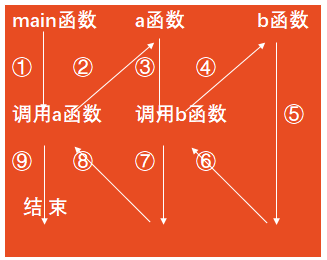
\includegraphics[scale=0.3]{main-a-b}
\column{0.5\textwidth}
\begin{lstlisting}[frame=leftline]
int a()
{
    int c; // 与main()中的c无关
    ...;
    c=b();// 函数调用
    ...;
    return c;
}
int b()
{
    ...;
    return 10;
}
\end{lstlisting}
\end{columns}
\medskip
\end{frame}


\begin{frame}[shrink,fragile]{例: 求4个整数中的最大者。}
\begin{columns}[T]
\column{0.54\textwidth}
\begin{lstlisting}
#include<stdio.h> 
int max2(int x,int y);
int max4(int a,int b,int c,int d); 
int main() // 主函数
{
   int a=b,c,d;
   scanf("%d%d%d%d",&a,&b,&c,&d);
   printf("较大者=%d\n", max4(a,b,c,d));
   printf("较大者=%d\n", max2(max2(a,b),max2(c,d))); // 等效
   return 0; 
}
\end{lstlisting}
\column{0.47\textwidth}
\begin{lstlisting}[frame=leftline]
// 定义函数
int max2(int x,int y) // 形式参数
{  
   int z;
   z=x>y ? x : y;
   return z; 
}
int max4(int a,int b,int c,int d)
{
  return max2(max2(a,b),max2(c,d));
}
\end{lstlisting}
\end{columns}
~\\
\end{frame}

\section{函数的递归调用}

\begin{frame}[shrink,fragile]{函数的递归调用}
在调用一个函数的过程中又出现直接或间接地调用该函数本身,称为函数的递归调用。
\begin{columns}[T]
\column{0.4\textwidth}
\begin{lstlisting}
// 递推公式: f(0)=0,f(1)=1, 
//     n>1: f(n)=n+f(n-1)
int f(int n) 
{
   int sum;
   if(n==0||n==1) sum=n;
   else sum=n+f(n-1); 
   return sum; 
}
\end{lstlisting}
\column{0.4\textwidth}
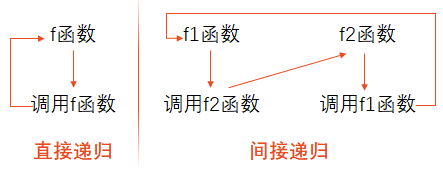
\includegraphics[scale=0.35]{recursion}
\end{columns}
程序中不应出现无终止的递归调用,而只应出现\textbf{有限次数的,有终止的递归调用},这可以用if语句来控制,只有在某一条件成立时才继续执行递归调用;否则就不再继续。
\end{frame}

\begin{frame}[shrink,fragile]{递归调用过程分析(push)}
\vspace{-0.2cm}
\begin{lstlisting}
// 递推公式: f(0)=0,f(1)=1, n>1: f(n)=n+f(n-1)
int f(int n) 
{
  int sum;
  if(n==0||n==1) sum=n;
  else sum=n+f(n-1); // 未完成的计算用"栈"存储起来(push)
  return sum; // 函数return前,从"栈"顶取数据,计算,直到"栈"空
}
\end{lstlisting}
系统内部自动维护一个称作``栈"的存储数据的空间,栈是一种``先进后出(FILO)=后进先出(LIFO)"的数据结构。向栈中存储数据操作称作push, 取出栈顶数据操作称作pop。第一个push的数据,最后一个被pop.
\begin{columns}[T]
\column{0.2\textwidth}<1->
\begin{tabular}{|c|}
	\hline 
	\rowcolor{yellow}f(5)=5+f(4) \\ 
	\hline 
\end{tabular}\\ 
栈[push(n=5)]
\column{0.2\textwidth}<2->
\begin{tabular}{|c|}
	\hline 
	\rowcolor{yellow}f(4)=4+f(3) \\ 
	\hline 
	f(5)=5+f(4) \\ 
	\hline 
\end{tabular}\\ 
栈[push(n=4)]
\column{0.2\textwidth}<3->
\begin{tabular}{|c|}
	\hline 
	\rowcolor{yellow}f(3)=3+f(2) \\ 
	\hline 
	f(4)=4+f(3) \\ 
	\hline 
	\hline 
	f(5)=5+f(4) \\ 
	\hline 
\end{tabular}\\ 
栈[push(n=3)]
\column{0.2\textwidth}<4->
\begin{tabular}{|c|}
	\hline 
	\rowcolor{yellow}f(2)=2+f(1) \\ 
	\hline 
	f(3)=3+f(2) \\ 
	\hline 
	f(4)=4+f(3) \\ 
	\hline 
	\hline 
	f(5)=5+f(4) \\ 
	\hline 
\end{tabular}\\ 
栈[push(n=2)]
\end{columns}
~\\
\end{frame}

\begin{frame}[shrink,fragile]{递归调用过程分析(pop)}
\vspace{-0.2cm}
\begin{lstlisting}
// 递推公式: f(0)=0,f(1)=1, n>1: f(n)=n+f(n-1)
int f(int n) 
{
  int sum;
  if(n==0||n==1) sum=n;
  else sum=n+f(n-1); // 未完成的计算用"栈"存储起来(push)
  return sum; // 函数return前,从"栈"顶取数据,计算,直到"栈"空
}
\end{lstlisting}
系统内部自动维护一个称作``栈"的存储数据的空间,栈是一种``先进后出(FILO)=后进先出LIFO"的数据结构。向栈中存储数据操作称作push, 取出数据操作称作pop。第一个push的数据,最后一个被pop.
\begin{columns}[T]
	\column{0.25\textwidth}<4->
	\begin{tabular}{|c|}
		\hline 
		\rowcolor{yellow}f(5)=5+f(4) \\ 
		\hline 
	\end{tabular}\\ 
	栈[pop(n=5)]\\
	f(5)=5+f(4)=15
	\column{0.25\textwidth}<3->
	\begin{tabular}{|c|}
		\hline 
		\rowcolor{yellow}f(4)=4+f(3) \\ 
		\hline 
		f(5)=5+f(4) \\ 
		\hline 
	\end{tabular}\\ 
	栈[pop(n=4)]\\
	f(4)=4+f(3)=10
	\column{0.25\textwidth}<2->
	\begin{tabular}{|c|}
		\hline 
		\rowcolor{yellow}f(3)=3+f(2) \\ 
		\hline 
		f(4)=4+f(3) \\ 
		\hline 
		\hline 
		f(5)=5+f(4) \\ 
		\hline 
	\end{tabular}\\ 
	栈[pop(n=3)]\\
	f(3)=3+f(2)=6
	\column{0.25\textwidth}<1->
	\begin{tabular}{|c|}
		\hline 
		\rowcolor{yellow}f(2)=2+f(1) \\ 
		\hline 
		f(3)=3+f(2) \\ 
		\hline 
		f(4)=4+f(3) \\ 
		\hline 
		\hline 
		f(5)=5+f(4) \\ 
		\hline 
	\end{tabular}\\ 
	栈[pop(n=2)]\\
	f(2)=2+f(1)=3
\end{columns}
~\\
\end{frame}

\begin{frame}[shrink]{例: age(n)}
有5个学生坐在一起,问第5个学生多少岁,他说比第4个学生大2岁。问第4个学生岁数,他说比第3个学生大2岁。问第3个学生,又说比第2个学生大2岁。问第2个学生,说比第1个学生大2岁。最后问第1个学生,他说是10岁。请问第5个学生多大。
~\\
\pause
\[ \text{第n个学生年龄 }
\begin{cases}
age(n)=10         & (n=1)\\
age(n)=age(n-1)+2 & (n>1) 
\end{cases}
\]
\end{frame}

\begin{frame}[shrink,fragile]{例: age(n), 递归调用过程分析(push)}
\vspace{-0.2cm}
\begin{lstlisting}
// 递推公式: age(1)=10; n>1: age(n)=age(n-1)
int age(int n) 
{
  int y;
  if(n==1) y=10;
  else y=age(n-1)+2; // 未完成的计算用"栈"存储起来(push)
  return y; // 函数return前,从"栈"顶取数据,计算,直到"栈"空
}
\end{lstlisting}
压栈: push
\begin{columns}[T]
	\column{0.2\textwidth}<1->
	\begin{tabular}{|c|}
		\hline 
		\rowcolor{yellow}age(5)=age(4)+2 \\ 
		\hline 
	\end{tabular}\\ 
	栈[push(n=5)]
	\column{0.2\textwidth}<2->
	\begin{tabular}{|c|}
		\hline 
		\rowcolor{yellow}age(4)=age(3)+2 \\ 
		\hline 
		age(5)=age(4)+2 \\ 
		\hline 
	\end{tabular}\\ 
	栈[push(n=4)]
	\column{0.2\textwidth}<3->
	\begin{tabular}{|c|}
		\hline 
		\rowcolor{yellow}age(3)=age(2)+2 \\ 
		\hline 
		age(4)=age(3)+2 \\ 
		\hline 
		\hline 
		age(5)=age(4)+2 \\ 
		\hline 
	\end{tabular}\\ 
	栈[push(n=3)]
	\column{0.2\textwidth}<4->
	\begin{tabular}{|c|}
		\hline 
		\rowcolor{yellow}age(2)=age(1)+2 \\ 
		\hline 
		age(3)=age(2)+2 \\ 
		\hline 
		age(4)=age(3)+2 \\ 
		\hline 
		\hline 
		age(5)=age(4)+2 \\ 
		\hline 
	\end{tabular}\\ 
	栈[push(n=2)]
\end{columns}
~\\
\end{frame}

\begin{frame}[shrink,fragile]{例: age(n), 递归调用过程分析(pop)}
\vspace{-0.2cm}
\begin{lstlisting}
// 递推公式: age(1)=10; n>1: age(n)=age(n-1)
int age(int n) 
{
  int y;
  if(n==1) y=10;
  else y=age(n-1)+2; // 未完成的计算用"栈"存储起来(push)
  return y; // 函数return前,从"栈"顶取数据,计算,直到"栈"空
}
\end{lstlisting}
弹出: pop
\begin{columns}[T]
\column{0.25\textwidth}<4->
\begin{tabular}{|c|}
	\hline 
	\rowcolor{yellow}age(5)=age(4)+2 \\ 
	\hline 
\end{tabular}\\ 
栈[pop(n=5)]\\
age(5)=age(4)+2=18
\column{0.25\textwidth}<3->
\begin{tabular}{|c|}
	\hline 
	\rowcolor{yellow}age(4)=age(3)+2 \\ 
	\hline 
	age(5)=age(4)+2 \\ 
	\hline 
\end{tabular}\\ 
栈[pop(n=4)]\\
age(4)=age(3)+2=16
\column{0.25\textwidth}<2->
\begin{tabular}{|c|}
	\hline 
	\rowcolor{yellow}age(3)=age(2)+2 \\ 
	\hline 
	age(4)=age(3)+2 \\ 
	\hline 
	\hline 
	age(5)=age(4)+2 \\ 
	\hline 
\end{tabular}\\ 
栈[pop(n=3)]\\
age(3)=age(2)+2=14
\column{0.25\textwidth}<1->
\begin{tabular}{|c|}
	\hline 
	\rowcolor{yellow}age(2)=age(1)+2 \\ 
	\hline 
	age(3)=age(2)+2 \\ 
	\hline 
	age(4)=age(3)+2 \\ 
	\hline 
	\hline 
	age(5)=age(4)+2 \\ 
	\hline 
\end{tabular}\\ 
栈[pop(n=2)]\\
age(2)=age(1)+2=12
\end{columns}
~\\
\end{frame}

\begin{frame}[shrink,fragile]{例: $n!$}
\vspace{-0.3cm}
\begin{tikzpicture}
\node[text width=\textwidth] (a) {
\begin{lstlisting}
double fac(int n) // n!较大,因此函数返回类型设置为double
{
   if(n==0 || n==1) return 1;
   else return n*fac(n-1);
}
int main()                   
{  
   printf("%.0lf\n",fac(2)); // 2
   printf("%.0lf\n",fac(3)); // 6
   printf("%.0lf\n",fac(4)); // 24
   printf("%.0lf\n",fac(20));// 2432902008176640000
   return 0;           
}           
\end{lstlisting}
};
\node[anchor=north east] at($(a.north east)+(-2,-2)$) {
	$n!=\begin{cases}
	1 &(n=0,1)\\
	n(n-1) &(n>1)
	\end{cases}$
};
\end{tikzpicture}
\end{frame}

\begin{frame}[shrink,fragile]{例: 斐波那契数列}
\vspace{-0.3cm}
\begin{tikzpicture}
\node[text width=\textwidth] (a) {
\begin{lstlisting}
double F(int n) // Fn较大,因此函数返回类型设置为double
{
   if(n==0 || n==1) return 1;
   else return F(n-1)+F(n-2);
}
int main()                   
{  
   int i;
   for(i=0;i<20;i++)
   {
      printf("%d\t",(int)F(i));
      if((i+1)%4==0) printf("\n");
   } 
   return 0;           
}                            
\end{lstlisting}
};
\node[anchor=north east] at($(a.north east)+(-2,-2)$) {
$\begin{cases}
F_n=1 &(n=0,1)\\
F_n=F_{n-1}+F_{n-2} &(n>1)
\end{cases}$
};
\end{tikzpicture}
\end{frame}

\begin{frame}[shrink,fragile]{例: 数字处理}
编写一个程序,从键盘输入一个非零整数n(0 < n <= 1000000000),对整数n进行如下处理:\\
将整数的各位数字取出来相加,如果结果是一位数则输出该数,否则重复上述过程,直到得到的结果为一位数,并输出该结果。\\
例如:n=456,变换过程如下\\
4+5+6=15\\
1+5=6\\
输出结果为6
\end{frame}

\begin{frame}[shrink,fragile]{例: 数字处理---非递归实现}
\vspace{-0.3cm}
\begin{columns}[T]
\column{0.5\textwidth}
\begin{lstlisting}
#include<stdio.h>
int bitsSum(int a);
int main()
{
   int n,sum;
   scanf("%d",&n);
   while(1)
   {
      sum=bitsSum(n);
      if(sum<=9) break;//1位数字
      else n=sum; // 继续下一轮迭代 
    }
    printf("%d\n",sum); 
    return 0;
}
\end{lstlisting}
\column{0.4\textwidth}
\begin{lstlisting}[frame=leftline]
// 整数a的各位数字之和
int bitsSum(int a)
{
   int sum=0;
   while(a)
   {
      sum += a%10;
      a /= 10;
   }
   return sum;
}
\end{lstlisting}
\end{columns}
~\\
\end{frame}

\begin{frame}[shrink,fragile]{例: 数字处理---递归实现}
\vspace{-0.3cm}
\begin{columns}[T]
\column{0.4\textwidth}
\begin{lstlisting}
#include<stdio.h>
int bitsSum(int a);
int bits1(int n);

int main()
{
   int n,sum=0;
   scanf("%d",&n);
   printf("%d\n",bits1(n)); 
   return 0;
} 
\end{lstlisting}
\column{0.6\textwidth}
\begin{lstlisting}[frame=leftline]
// 整数a的各位数字之和
int bitsSum(int a)
{
   int sum;
   if(a==0) sum=0;  
   else sum=bitsSum(a/10)+a%10;
   return sum;
}
// 确保最后是1位数字
int bits1(int n)
{
   int result;
   result=bitsSum(n);
   if(result>9) result=bits1(result);//递归
   return result; 
}
\end{lstlisting}
\end{columns}
~\\
\end{frame}

\begin{frame}[shrink,fragile]{例: 二进制输出(正序)}
\vspace{-0.3cm}
\begin{columns}[T]
\column{0.6\textwidth}
\begin{lstlisting}
void to_binary(unsigned long n);
int main()
{
  // 无符号长整型
  unsigned long x=0XD2; //11010010
  scanf("%x",&x); //十六进制输入
  //scanf("%uld",&x); //等效10进制无符号长整型  
  to_binary(x);
  putchar('\n'); 
  return 0;
}

void to_binary(unsigned long n)
{
  int r;
  r=n%2;//01001011
  // push(先计算的二进制位r)
  if(n>=2) to_binary(n/2); 
  // pop(后进先出FILO=先进后出FILO) 
  putchar('0'+r);//11010010
} 
\end{lstlisting}
\column{0.3\textwidth}
以\lstinline|x=0XD2|为例,分析递归过程。 \\
\lstinline|r=n%2;|\\
计算$2^0,2^1,\dots,2^7$
\begin{tabular}{|c|c|c|c||c|c|c|c|}
	\hline 
	$2^0$& $2^1$ & $2^2$ & $2^3$ & $2^4$ & $2^5$ & $2^6$ & $2^7$  \\ 
	\hline 
	0 & 1 & 0 & 0 & 1 & 0 & 1 & 1 \\ 
	\hline 
\end{tabular}
~\\
\lstinline|to_binary(n/2);|\\
push(先计算的r),栈顶(top,最左端), 栈底(bottom,最右端) 
\begin{tabular}{|c|c|c|c||c|c|c|c|}
	\hline 
	$2^7$& $2^6$ & $2^5$ & $2^4$ & $2^3$ & $2^2$ & $2^1$ & $2^0$
	\\ 
	\hline 
	1 & 1 & 0 & 1 & 0 & 0 & 1 & 0 \\ 
	\hline 
\end{tabular}  
~\\
\lstinline|putchar('0'+r);|\\
pop(后进先出), 即栈顶元素先出,栈底元素最后出
\begin{tabular}{|c|c|c|c||c|c|c|c|}
	\hline 
	$2^7$& $2^6$ & $2^5$ & $2^4$ & $2^3$ & $2^2$ & $2^1$ & $2^0$
	\\ 
	\hline 
	1 & 1 & 0 & 1 & 0 & 0 & 1 & 0 \\ 
	\hline 
\end{tabular}  
\end{columns}
~\\
\end{frame}

\begin{frame}[shrink,fragile]{例: 二进制输出(倒序)}
\begin{columns}[T]
\column{0.6\textwidth}
\begin{lstlisting}
void to_binary(unsigned long n);
int main()
{
  // 无符号长整型
  unsigned long x=0XD2; //11010010
  scanf("%x",&x); //十六进制输入
  //scanf("%uld",&x); //等效10进制无符号长整型 
  to_binary(x);
  putchar('\n'); 
  return 0;
}

void to_binary(unsigned long n)
{
  int r;
  r=n%2;//01001011
  putchar('0'+r);//01001011
  // push(先计算的二进制位r)
  if(n>=2) to_binary(n/2); 
} 
\end{lstlisting}
\column{0.4\textwidth}
	以\lstinline|x=XD2|为例,分析递归过程。 \\
	\lstinline|r=n%2;|\\
	计算$2^0,2^1,\dots,2^7$
	\begin{tabular}{|c|c|c|c||c|c|c|c|}
		\hline 
		$2^0$& $2^1$ & $2^2$ & $2^3$ & $2^4$ & $2^5$ & $2^6$ & $2^7$  \\ 
		\hline 
		0 & 1 & 0 & 0 & 1 & 0 & 1 & 1 \\ 
		\hline 
	\end{tabular}
	~\\
	\lstinline|to_binary(n/2);|\\
	push(先计算的r),栈顶(top,最左端), 栈底(bottom,最右端) 
	\begin{tabular}{|c|c|c|c||c|c|c|c|}
		\hline 
		$2^7$& $2^6$ & $2^5$ & $2^4$ & $2^3$ & $2^2$ & $2^1$ & $2^0$
		\\ 
		\hline 
		1 & 1 & 0 & 1 & 0 & 0 & 1 & 0 \\ 
		\hline 
	\end{tabular}  
	~\\
	pop(后进先出), 即栈顶元素先出,栈底元素最后出
	\begin{tabular}{|c|c|c|c||c|c|c|c|}
		\hline 
		$2^7$& $2^6$ & $2^5$ & $2^4$ & $2^3$ & $2^2$ & $2^1$ & $2^0$
		\\ 
		\hline 
		1 & 1 & 0 & 1 & 0 & 0 & 1 & 0 \\ 
		\hline 
	\end{tabular}  
\end{columns}
~\\
\end{frame}

\begin{frame}{例: Hanoi(汉诺)塔问题}
古代有一个梵塔,塔内有3个座A,B,C。开始时A座上有64个盘子,盘子大小不等,大的在下,小的在上。有一个老和尚想把这64个盘子从A座移到C座,但规定每次只允许移动一个盘,且在移动过程中在3个座上都始终保持大盘在下,小盘在上。在移动过程中可以利用B座。\\
要求编程序输出移动盘子的步骤。\\
~\\
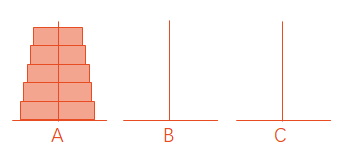
\includegraphics[scale=0.4]{Hanoi}
\end{frame}

\begin{frame}[shrink]{例: Hanoi(汉诺)塔问题---解题思路}
\begin{itemize}
	\item 老和尚想: 假如有第2个和尚将上面63个盘子从A座移到B座。我就能将64个盘子从A座移到C座。。
	\begin{enumerate}
		\item 命令第2个和尚将63个盘子从A座移到B座;
		\item 自己将1个盘子(最底下的、最大的盘子)从A座移到C座;
		\item 再命令第2个和尚将63个盘子从B座移到C座。
	\end{enumerate}
    \item 第2个和尚想: 假如有第3个和尚能将上面62个盘子从A座移到C座,我就能将63个盘子从A座移到B座。
    \begin{enumerate}
    	\item 命令第3个和尚将62个盘子从A座移到C座;
    	\item 自己将1个盘子从A座移到B座;
    	\item 再命令第3个和尚将62个盘子从C座移到B座。
    \end{enumerate}
    \item $\cdots$
\end{itemize}
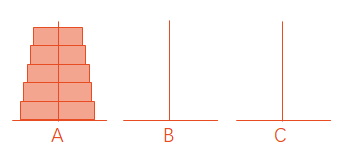
\includegraphics[scale=0.25]{Hanoi}
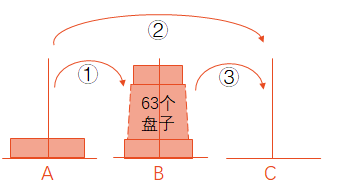
\includegraphics[scale=0.3]{Hanoi-1}
\end{frame}

\begin{frame}[shrink]{例: Hanoi(汉诺)塔问题---解题思路(3层)}
\begin{columns}[T]
	\column{0.6\textwidth}
	\begin{itemize}
		\item 将A座的3个盘子移到C座, 分3步:
		\begin{enumerate}
			\item 将A上2个盘子移到B\textbf{(借助C座)}。
			\item 将A上1个盘子移到C\textbf{(直接实现)}。
			\item 将B上2个盘子移到C\textbf{(借助A座)}。
		\end{enumerate}
	    \item 分解第1步: 将A上的2个盘子移到B:
	    \begin{enumerate}
	    	\item 将A上1个盘子移到C\textbf{(借助C座)}。
	    	\item 将A上1个盘子移到B。
	    	\item 将C上1个盘子移到B。
	    \end{enumerate}
        \item 分解第3步: 将B座的2个盘子移到C座:
        \begin{enumerate}
        	\item 将B上1个盘子移到A\textbf{(借助A座)}。
        	\item 将B上1个盘子移到C。
        	\item 将A上1个盘子移到C。
        \end{enumerate}
	\end{itemize}
	\column{0.4\textwidth}
	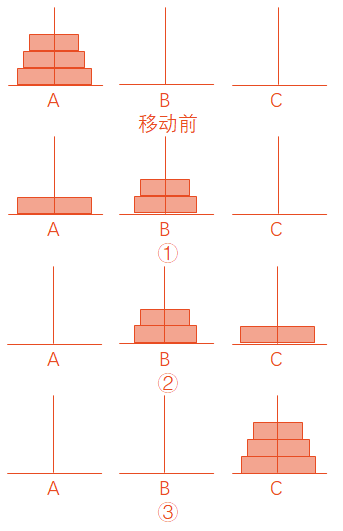
\includegraphics[scale=0.3]{Hanoi-2}
\end{columns}
~\\
\end{frame}

\begin{frame}[shrink,fragile]{例: Hanoi(汉诺)塔问题---解}
\begin{columns}[T]
\column{0.4\textwidth}
\begin{lstlisting}
void hanoi(int n,char one,char two,char three);
void move(char one,char two);
int main()
{
   int n=3;
   scanf("%d",&n);
   //n个盘由'A'移到'C',借助'B'
   hanoi(n,'A','B','C');
   return 0;
}
void move(char one,char two)
{
 printf("%c->%c\n",one,two);
}
\end{lstlisting}
\column{0.6\textwidth}
\begin{lstlisting}[frame=leftline]
//将n个盘从one移到three,借助two
void hanoi(int n,char one,char two,char three)
{
   if(n==1) move(one,three); 
   else
   {
      //n-1盘从one移到two,借three
      hanoi(n-1,one,three,two); 
      //将1个盘从one移到three
      move(one,three); 
      //n-1盘从two移到three,借one
      hanoi(n-1,two,one,three); 
   }
}
\end{lstlisting}
\end{columns}
~\\
\end{frame}

\begin{frame}[shrink, fragile]%{例: Hanoi(汉诺)塔问题---分析代码(3层)}
\begin{columns}[T]
\column{0.4\textwidth}
	\begin{itemize}
		\small
		\item 将A座的3个盘子移到C座, 分3步:
		\begin{enumerate}
			\scriptsize
			\item 将A上2个盘子移到B\textbf{(借C)}。
			\item 将A上1个盘子移到C\textbf{(直接)}。
			\item 将B上2个盘子移到C\textbf{(借A)}。
		\end{enumerate}
		\item 分解第1步: 将A上的2个盘子移到B:
		\begin{enumerate}\scriptsize
			\item 将A上1个盘子移到C\textbf{(借C)}。
			\item 将A上1个盘子移到B。
			\item 将C上1个盘子移到B。
		\end{enumerate}
		\item 分解第3步: 将B座的2个盘子移到C座:
		\begin{enumerate}\scriptsize
			\item 将B上1个盘子移到A\textbf{(借A)}。
			\item 将B上1个盘子移到C。
			\item 将A上1个盘子移到C。
		\end{enumerate}
	\end{itemize}
\column{0.6\textwidth}
\begin{lstlisting}[frame=leftline]
//将n个盘从one移到three,借助two
void hanoi(int n,char one,char two,char three)
{
  if(n==1) move(one,three); // 递归终止条件, 出栈pop(2,...,n-1,n), 回归,回溯
  else
  { // 压栈push(n,n-1,n-2,...2)
    //n-1盘从one移到two,借three
    hanoi(n-1,one,three,two); 
    //将1个盘从one移到three
    move(one,three); 
    //n-1盘从two移到three,借one
    hanoi(n-1,two,one,three);
  }
}
\end{lstlisting}
\end{columns}
\textcolor{blue}{$A\to C,A\to B,C\to B,A\to C,B\to A,B\to C,A\to C$}\\
\end{frame}

\begin{frame}[shrink,fragile]{递归小结}
\begin{itemize}
	\item 递归函数必须满足两个条件:
	\begin{enumerate}
		\item 在每一次调用自己时,必须是(在某种意义上)更接近于解;
		\item 必须有一个终止处理的语句。
	\end{enumerate}
    \item 递归能够解决的问题:
    \begin{enumerate}
    	\item 数据的定义是按递归定义的。如Fibonacci函数。
    	\item 问题解法按递归算法实现。如Hanoi问题。
    	\item 数据的结构形式是按递归定义的。如二叉树、广义表等。
    \end{enumerate}
	\item 使用递归的关键在于将问题分解为小部分,递归不能永远进行下去,因为它总是以最小可能性问题结束,
	\item 递归函数的优点是定义简单,逻辑清晰,但是代码难于理解。
	\item 理论上,所有的递归函数都可以写成循环的方式,但循环逻辑不如递归清晰。
	\item 层次越深, 调用栈(内存)越大, 效率越低, 并且可能会溢出。因此, 能用循环解决的问题, 尽量不要用递归。
\end{itemize}
\end{frame}

\section{局部变量和全局变量}

\begin{frame}[shrink,fragile]{局部变量及其作用域}
定义在函数内部或复合语句中的变量称为\textbf{局部变量}。局部变量的\textbf{作用域}是从定义语句开始至函数或复合语句结束,不会影响作用域以外的同类型的同名变量值。 
\begin{columns}[T]
\column{0.5\textwidth}
\begin{lstlisting}
// 各函数中的局部变量, 不会相互影响。
float f1(folat a) 
{
   float c; // 本函数局部变量
   ....;
}
float f2(float a)
{ 
   float c; // 本函数局部变量
   ....;
}
int main()
{
   float c=10,d; // 本函数局部变量
   d=f1(c);
   d=f2(d);
}
\end{lstlisting}
\column{0.5\textwidth}
\begin{lstlisting}[frame=leftline]
// 各复合语句中的局部量, 不会相互影响。
float f1(folat a) 
{
   float c; // 本函数局部变量
   for(i=0;i<10;i++) 
   {
     int t; // 复合语句中的局部变量 
     ....
   }
   if(c>10)
   {
     int t; // 复合语句中的局部变量 
     ....
   }
   ...
}
\end{lstlisting}
\end{columns}
~\\
\end{frame}

\begin{frame}[shrink,fragile]{形式参数被当作本函数的局部变量}
形式参数被当作本函数的局部变量,因此它不会影响实际参数的值。
\begin{columns}[T]
\column{0.5\textwidth}
\begin{lstlisting}
float f1(folat a) 
{
  float c; // 本函数内部的局部变量不得与形式参数同名
  a=30; // 改变形式参数的值不会影响实际参数的值
  ....;
}
int main()
{
   float c=10,d; // 本函数局部变量
   d=f1(c); // f1函数对形参的改变不会影响实参c的值
   float x[2]={0.1,0.2}; 
   f2(x); // 函数内部可以改变数组元素的值
   printf("%f,%f,%f\n",c,x[0],x[1]); // 10,10.1,10.2  
}
\end{lstlisting}
\column{0.5\textwidth}
\begin{lstlisting}[frame=leftline]
// 函数内部可以改变数组元素的值,但是对地址的改变不会影响实参的地址
float f2(folat a[]) 
{
  a[0]=10.1; // 对数组元素的改变,就是对实参数组元素的改变
  a[1]=10.2;
  a=a+1; // 对数组名(地址)的改变, 不会影响实参的地址。
  ...
}
\end{lstlisting}
\end{columns}
~\\
\end{frame}

\begin{frame}[shrink,fragile]{全局变量及其作用域}
定义在函数外部的变量称为\textbf{全局变量}。与模块化函数封装思想冲突,不推荐使用。全局变量的作用域是从定义语句开始至该文件结束,会影响作用域内的同类型的同名变量值。 
\begin{lstlisting}
int g=0; // 全局变量
float f1(folat a) 
{
  g=10; // 改变全局变量的值
  ....;
}
float f2(float a)
{ 
  g=20; // 改变全局变量的值
  ....;
}
int main()
{
   g=30; // 改变全局变量的值
   ....;
}
\end{lstlisting}
\end{frame}




